\documentclass{article}

\usepackage{a4wide}
\usepackage[utf8]{inputenc}
\usepackage[T1]{fontenc}
\usepackage[french]{babel}
\usepackage[babel=true]{csquotes} % guillemets français
\usepackage{graphicx}
\graphicspath{{Images/}}
\usepackage{color}
\usepackage{hyperref}
\hypersetup{colorlinks,linkcolor=,urlcolor=blue}
\usepackage{float}
\usepackage[lined,boxed,commentsnumbered, ruled,vlined,linesnumbered, french, frenchkw, onelanguage]{algorithm2e}
\usepackage{mathtools}
\usepackage{schemabloc}
\usepackage{amsmath}
\usepackage{amssymb}
\usepackage{minted}
\usepackage{xurl}

\newcommand{\N}{\mathbb{N}}
\newcommand{\R}{\mathbb{R}}
\newcommand{\Min}[1]{\min\limits_{#1}}
\newcommand{\Max}[1]{\max\limits_{#1}}

\title{Développement pour mobiles}
\author{Pierre Jaffuer \& Olivier Vee}
\date{\today}

\begin{document}
\maketitle % pour écrire le titre
\begin{figure}[H]
    \centering
    
\includegraphics[width=0.75\linewidth]{AppsLogo.png}
\end{figure}

%% Le résumé:
\begin{abstract}
Dans le cadre de l'UE "Développement pour mobiles", nous avons réalisé un jeu mobile intitulé "Super Démineur". 
Le jeu du démineur à été popularisé par Windows, le principe est simple : le joueur dispose d'une grille plus ou moins grande dont le but est de la déminer avec pour seul aide des numéros indiquant le nombre de mines adjacentes.
\end{abstract}

\newpage
\tableofcontents 
\newpage



\section{Introduction}
\subsection{Présentation}

Super Démineur est une version du jeu du démineur dans lequel le joueur peut également :
\begin{itemize}
    \item placer des drapeaux dans la grille pendant la partie pour indiquer la présence de bombe et l'empêcher de l'ouvrir par accident
    \item évaluer ses performances grâce à un système de score 
    \item voir sa progression grâce a un historique des statistiques de toutes ses parties
\end{itemize}

\begin{figure}[H]
    \centering
    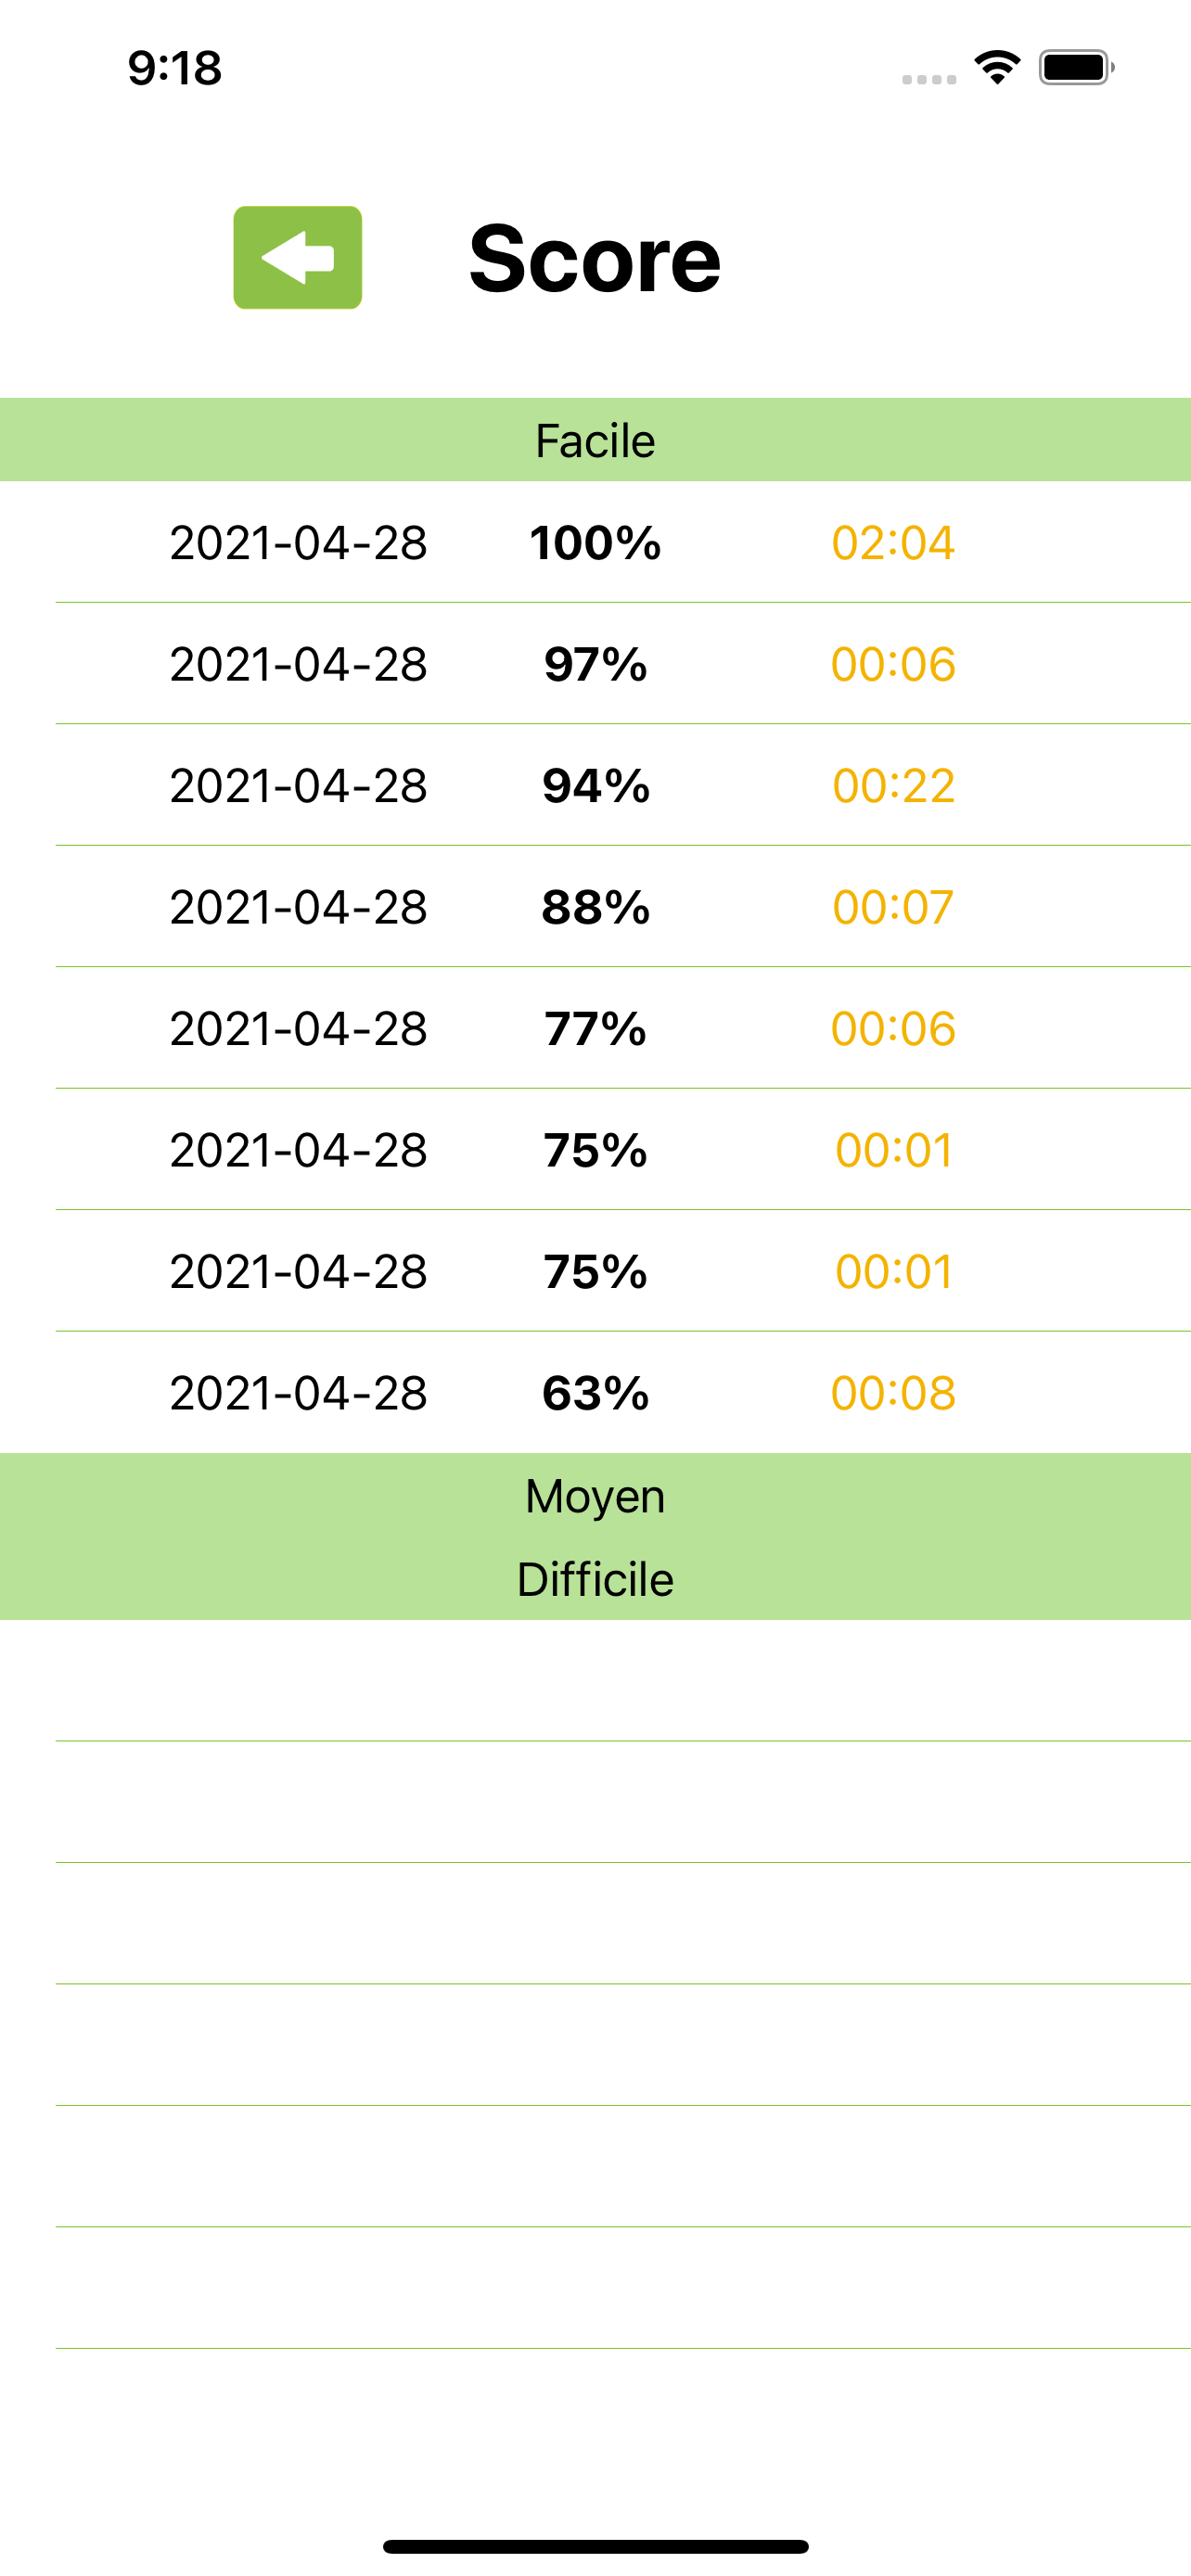
\includegraphics[width=0.3\linewidth]{ScoreView_iOs.png}
    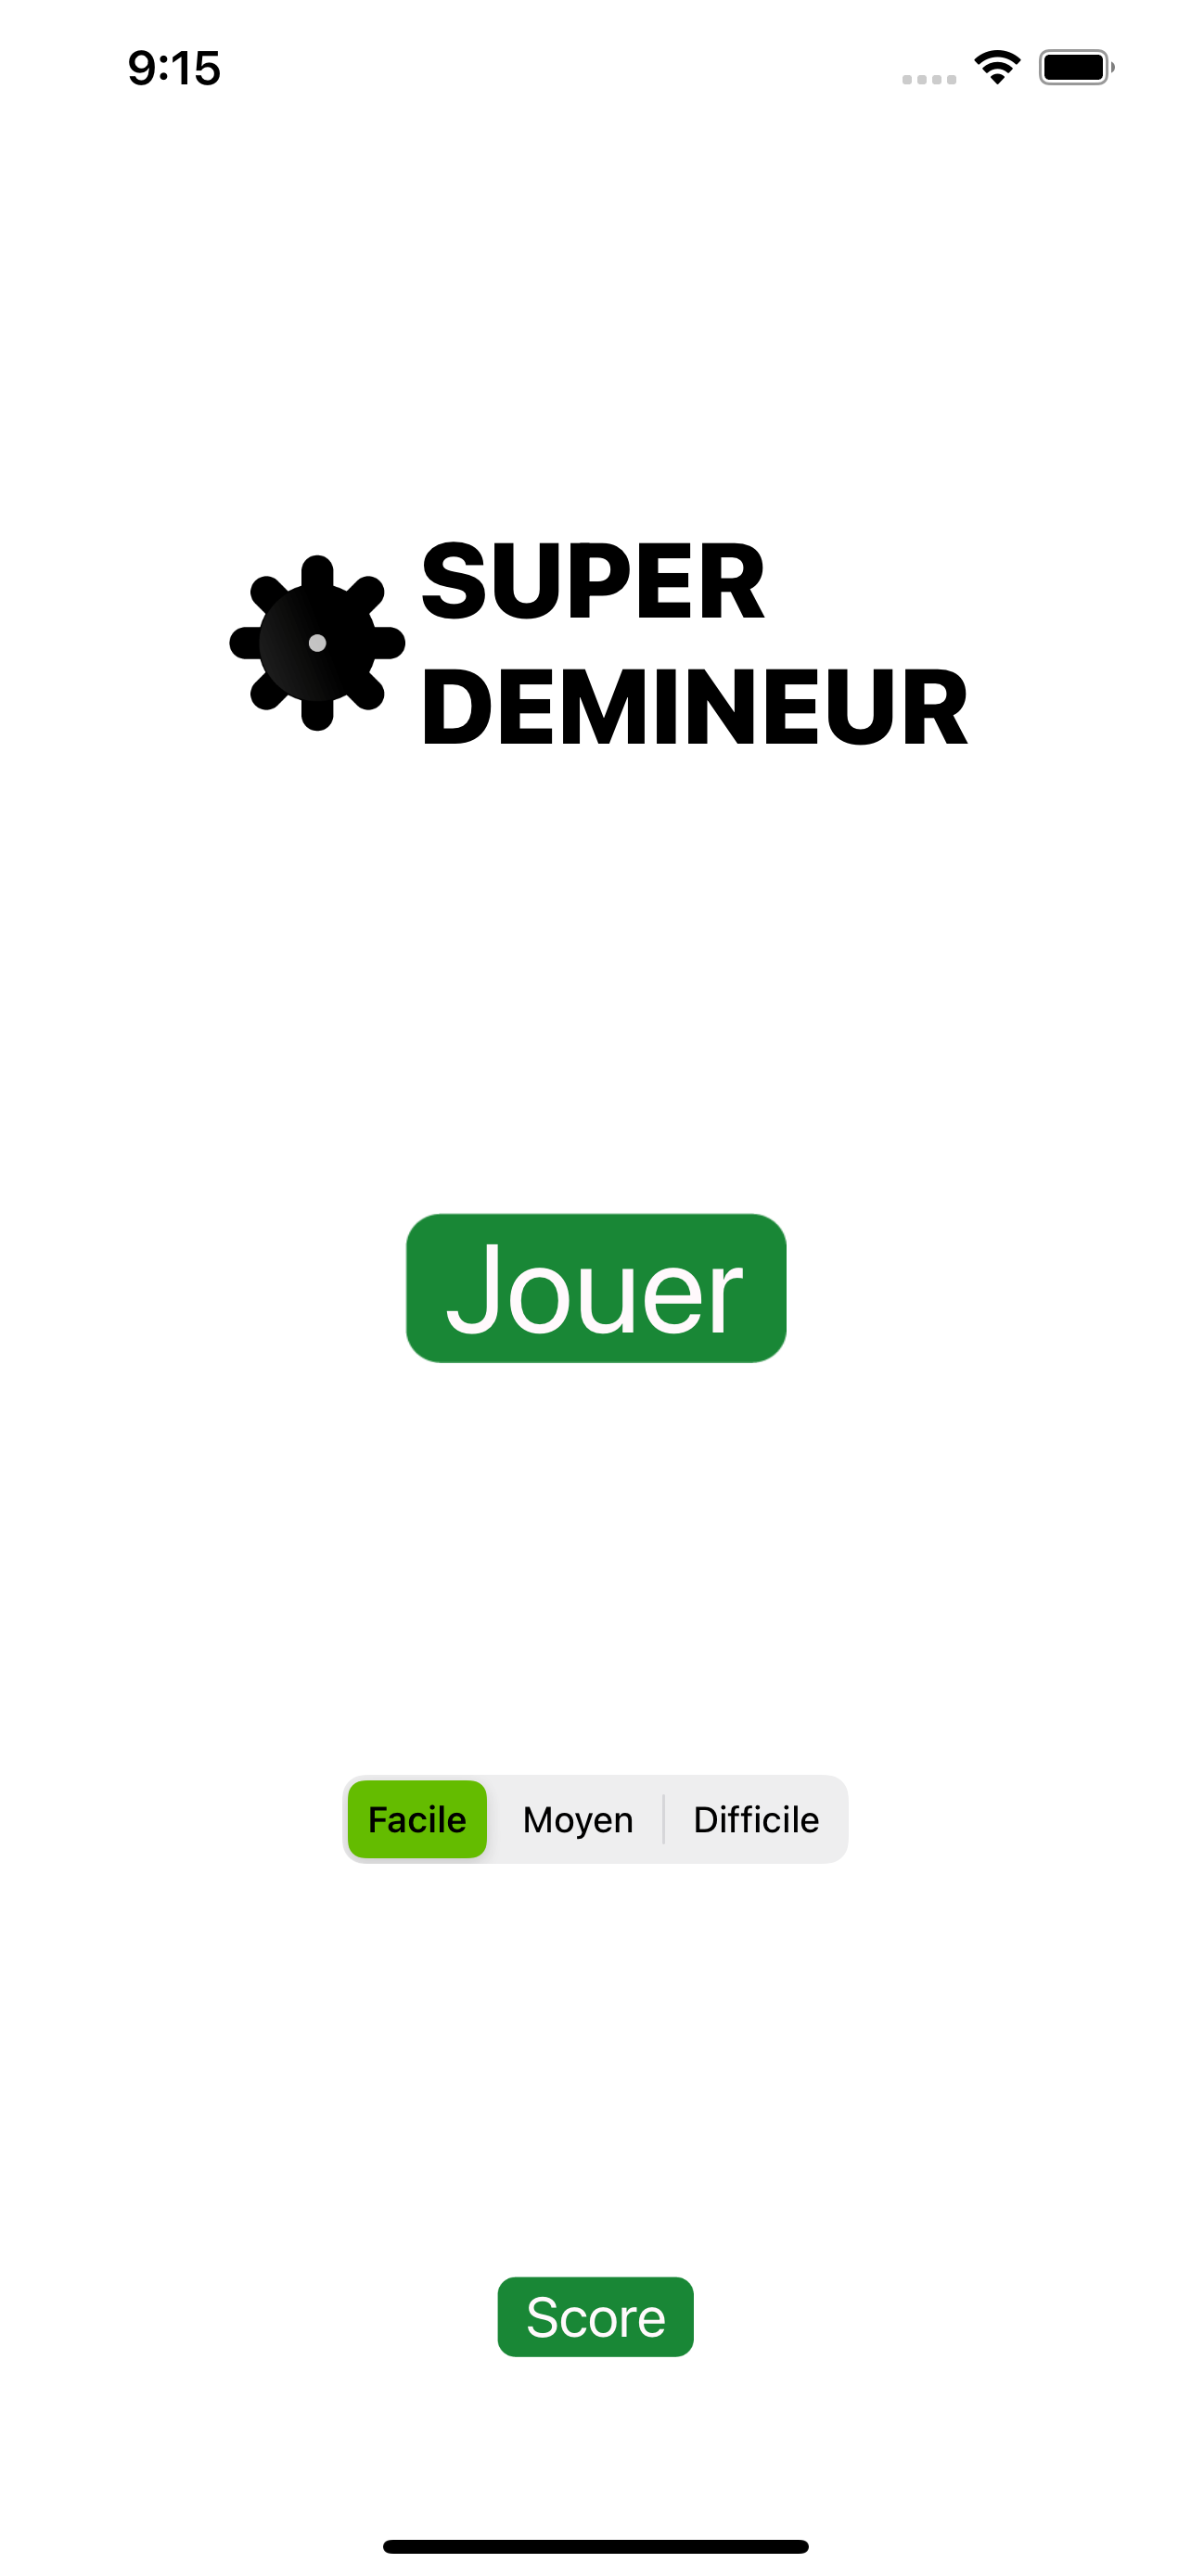
\includegraphics[width=0.3\linewidth]{MainView_iOs.png}
    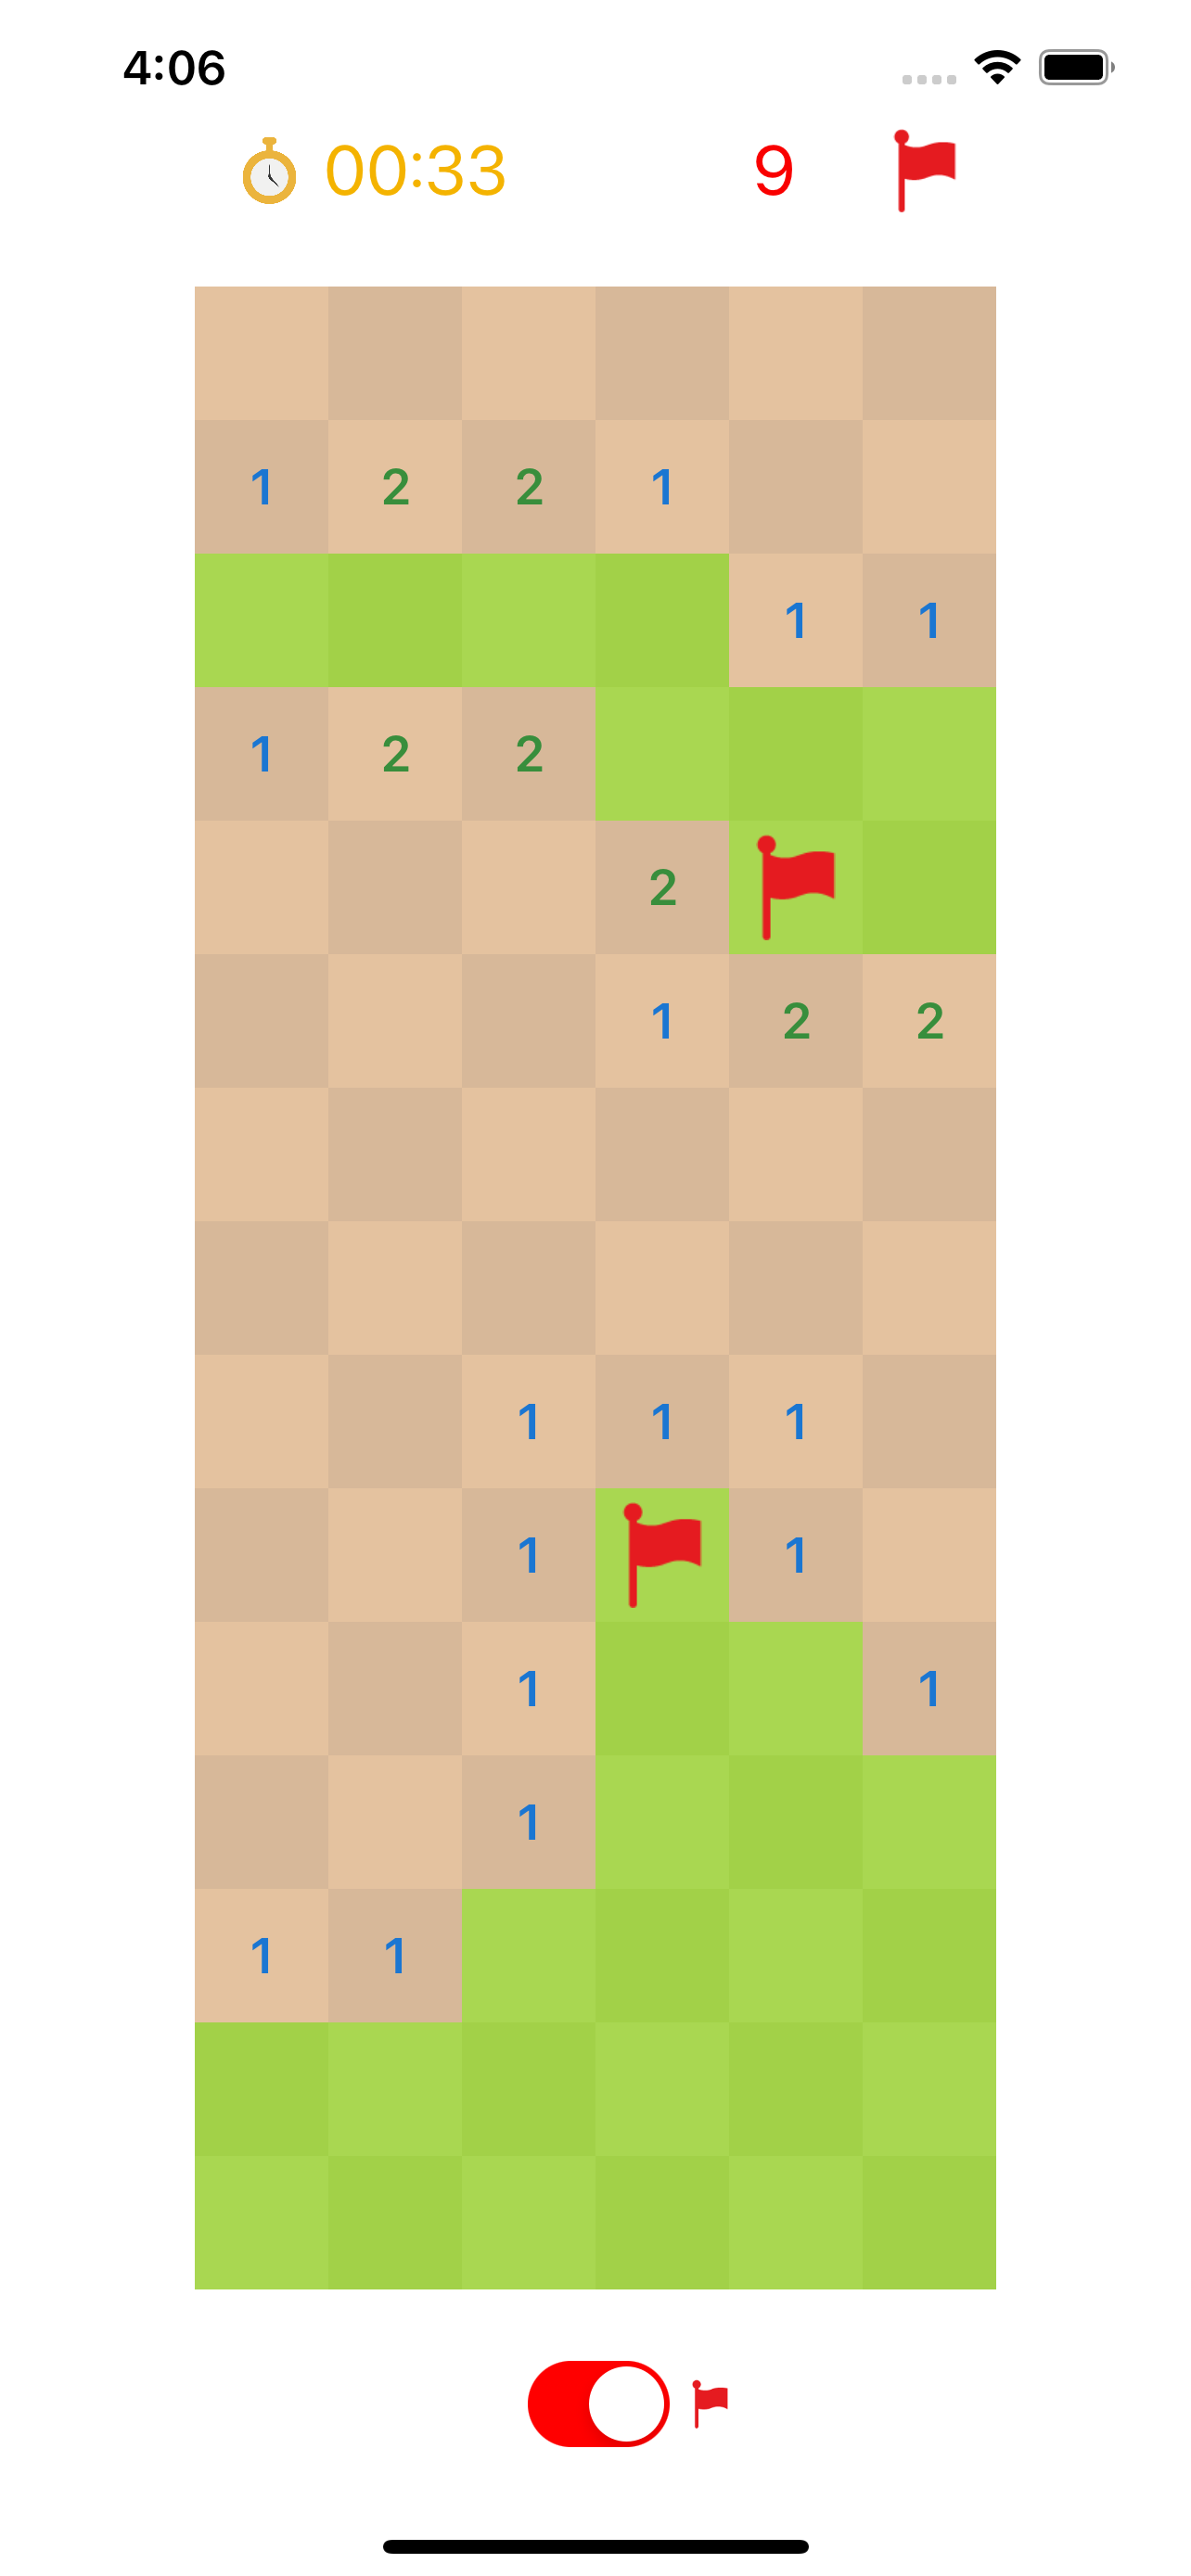
\includegraphics[width=0.3\linewidth]{Gameplay_iOs.png}
    \label{fig:figure1}
    \caption{De gauche à droite: la vue des scores, la vue principale, la vue du jeu}
\end{figure}

\subsection{Organisation}

Nous avons commencé par établir les solides fondations de ce projet :
\begin{itemize}
    \item  l'architecture UML commune à iOs et Android
    \item  les fonctionnalités clés de l'application émises précédemment 
    \item  le principe de fonctionnement de l'algorithme récursif de creusage 
    \item  la répartition des tâches 
\end{itemize}

Concernant la répartition des tâches, nous avons respectivement chacun développé une 
application : 
\begin{itemize}
    \item  la version Android pour Pierre (\url{https://github.com/smallcluster/Demineur})
    \item  la version iOs pour Olivier (\url{https://github.com/Rprojet/Demineur})
\end{itemize}

\subsection{Inspirations}
Pour le design du jeu, nous nous somme inspiré du démineur web de Google (disponible en cherchant "démineur" depuis le moteur de recherche).

\begin{figure}[H]
    \centering
    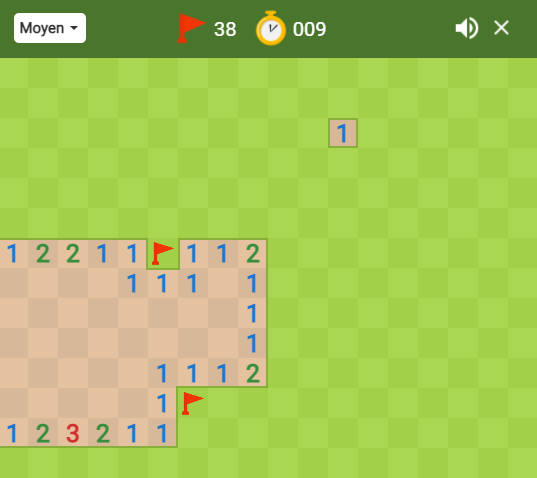
\includegraphics[width=0.7\linewidth]{demineurGoogle.png}
    \caption{Démineur web de google}
\end{figure}

Après avoir déterminé les différentes couleurs, Olivier a réalisé les ressources graphiques nécessaires sur Adobe Illustrator.

\begin{figure}[H]
    \centering
    
\includegraphics[width=0.1\linewidth]{flag.png}
    
\includegraphics[width=0.1\linewidth]{flag_disabled.png}
    
\includegraphics[width=0.1\linewidth]{mine.png}
    
\includegraphics[width=0.1\linewidth]{horloge.png}
    \caption{Les images créées par Olivier pour le projet}
\end{figure}

\section{Socle commun}

\subsection{Le diagramme UML}
\begin{figure}[H]
    \centering
    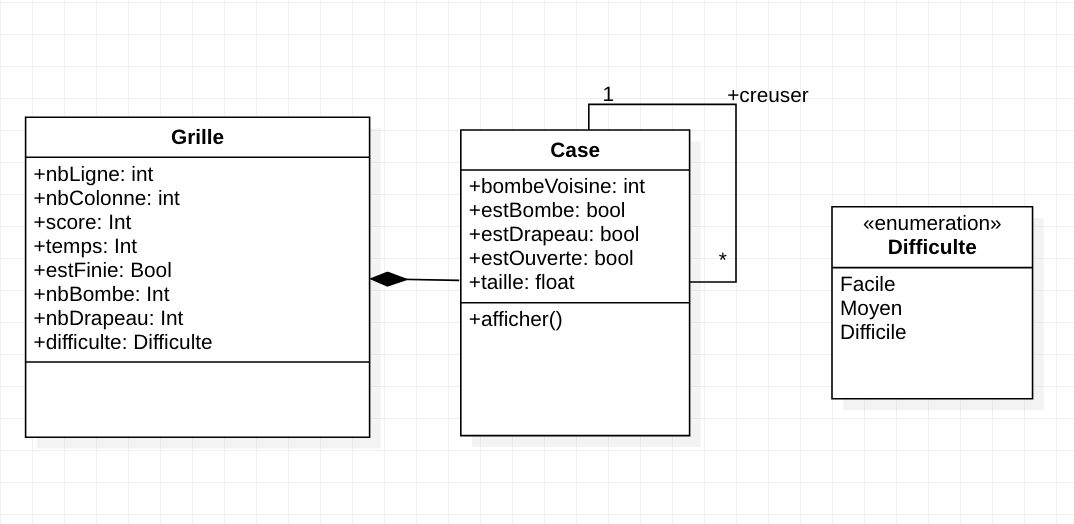
\includegraphics[width=0.7\linewidth]{Diagramme_UML.png}
    \caption{Diagramme UML initial}
\end{figure}

Ci-dessus vous trouverez les classes au coeur du gameplay de Super Démineur: 
\begin{itemize}
    \item  la classe "Case" ayant plusieurs états (bombe, vide etc..) et changeant son état suivant les cases sélectionnés par le joueur et la disposition de la grille. 
    \item  la classe "Grille" servant à la fois de modèle car elle agrège les objets Cases, mais aussi de contrôleur car elle gère le déroulement de la partie (initialisation de la partie paramétré par la difficulté, stockage du score de la fin de la partie, etc..)
\end{itemize}

\paragraph{\underline{Remarque:}}Le modèle UML n'est pas représentatif de l' implémentation finale du jeu, il a été réalisé au commencement du projet pour servir de guide.

\subsection{L'algorithme récursif de creusage}

Le jeu du Démineur implémente le principe suivant : "lorsque le joueur clique sur une case qui ne contient pas une bombe, alors cette case ouvre toutes les autres cases voisines (Von Neuman) qui ne contiennent elles-même pas de bombe dans leur voisinages (Moore ordre 1)". 
Au vue de l'énoncer de cette mécanique de jeu, c'est donc naturel quelle sera développer par une fonction récursive qui est la suivante:\\

\begin{algorithm}[H]
	\KwIn{$c_{i,j}$ la case à creuser de coordonnées $(i,j)$}
	// Cas de base:\\
	\If{$c_{i,j}$ est une bombe \textbf{ou} possède un drapeau}{
	    \Return{}
	}\uElseIf{$c_{i,j}$ a des bombes dans son voisinage de Moore d'ordre 1 }{
	    ouvrir($c_{i,j}$)\\
	    \Return{}
	}
	// Cas récursif: C'est une case vide\\
	ouvrir($c_{i,j}$)\\
	// Creuser les cases dans son voisinage de Von Neuman\\
	\If{$c_{i-1,j}$ est dans la grille}{
	    Creuser($c_{i-1,j}$)
	}
	\If{$c_{i+1,j}$ est dans la grille}{
	    Creuser($c_{i+1,j}$)
	}
	\If{$c_{i,j-1}$ est dans la grille}{
	    Creuser($c_{i,j-1}$)
	}
	\If{$c_{i,j+1}$ est dans la grille}{
	    Creuser($c_{i,j+1}$)
	}
	\caption{Creuser}
\end{algorithm}


\subsection{Taille de la grille}

Que ça soit pour iOs ou Android, sur une tablette ou un téléphone, l'application est homogène en terme de gameplay. C'est pourquoi, la dimension des cases dépendant de la taille de l'écran, le nombre de ligne de la grille sera déduit suivant l'accessibilité des cases sur les petits écrans. \\

Ainsi, nous avons retenus un nombre de ligne au maximum égale à 20 car au-delà, la dimension des lignes devenait inaccessible au tactile sur les petits écran. 
Pour ce qui du nombre de colonne, nous nous somme basés sur la définition standard la plus restrictive à savoir le 21/9. Ainsi pour un nombre l de ligne, le nombre c de colonne sera de :
$$c = \frac{9}{21} \times l$$

\subsection{Niveaux de difficultés}
En fonction de la difficulté choisie par l'utilisateur, le nombre de cases et la proportion des bombes sont modifiées. Puisque le nombre de colonnes se détermine à l'aide du nombre de lignes, on ne considère donc ici que le nombre de lignes et la proportion des bombes comme suit :\\

\begin{itemize}
    \item \textbf{Difficulté facile :} 10 lignes et 10 \% de bombes
    \item \textbf{Difficulté moyenne :} 15 lignes et 13 \% de bombes
    \item \textbf{Difficulté difficile :} 20 lignes et 15 \% de bombes
\end{itemize}


\subsection{Homogénéité entre iOs et Android}
Bien que la logique du fonctionnement de l'application soit différente entre la version iOs et Android, cela n'a aucun impact sur l'expérience utilisateur. En revanche, une interface différente entre les deux versions pourrait être mal perçu par ceux-ci, de ce fait, les interface des deux version doivent se ressembler le plus possible.\\

Cependant, certains composants natifs d'iOs n'existent pas sur Android et vice versa, nous nous sommes donc limité dans le choix des composants à utiliser. On s'est tout de même permis d'utiliser un \textit{SegmentedButton} sur iOs pour le choix de la difficulté pour des raisons esthétiques, ce composant n'étant pas disponible sur Android, nous l'avons émulé à l'aide d' un \textit{RadioGroup} via un style xml modifié \cite{segmented}.

\begin{figure}[H]
    \centering
    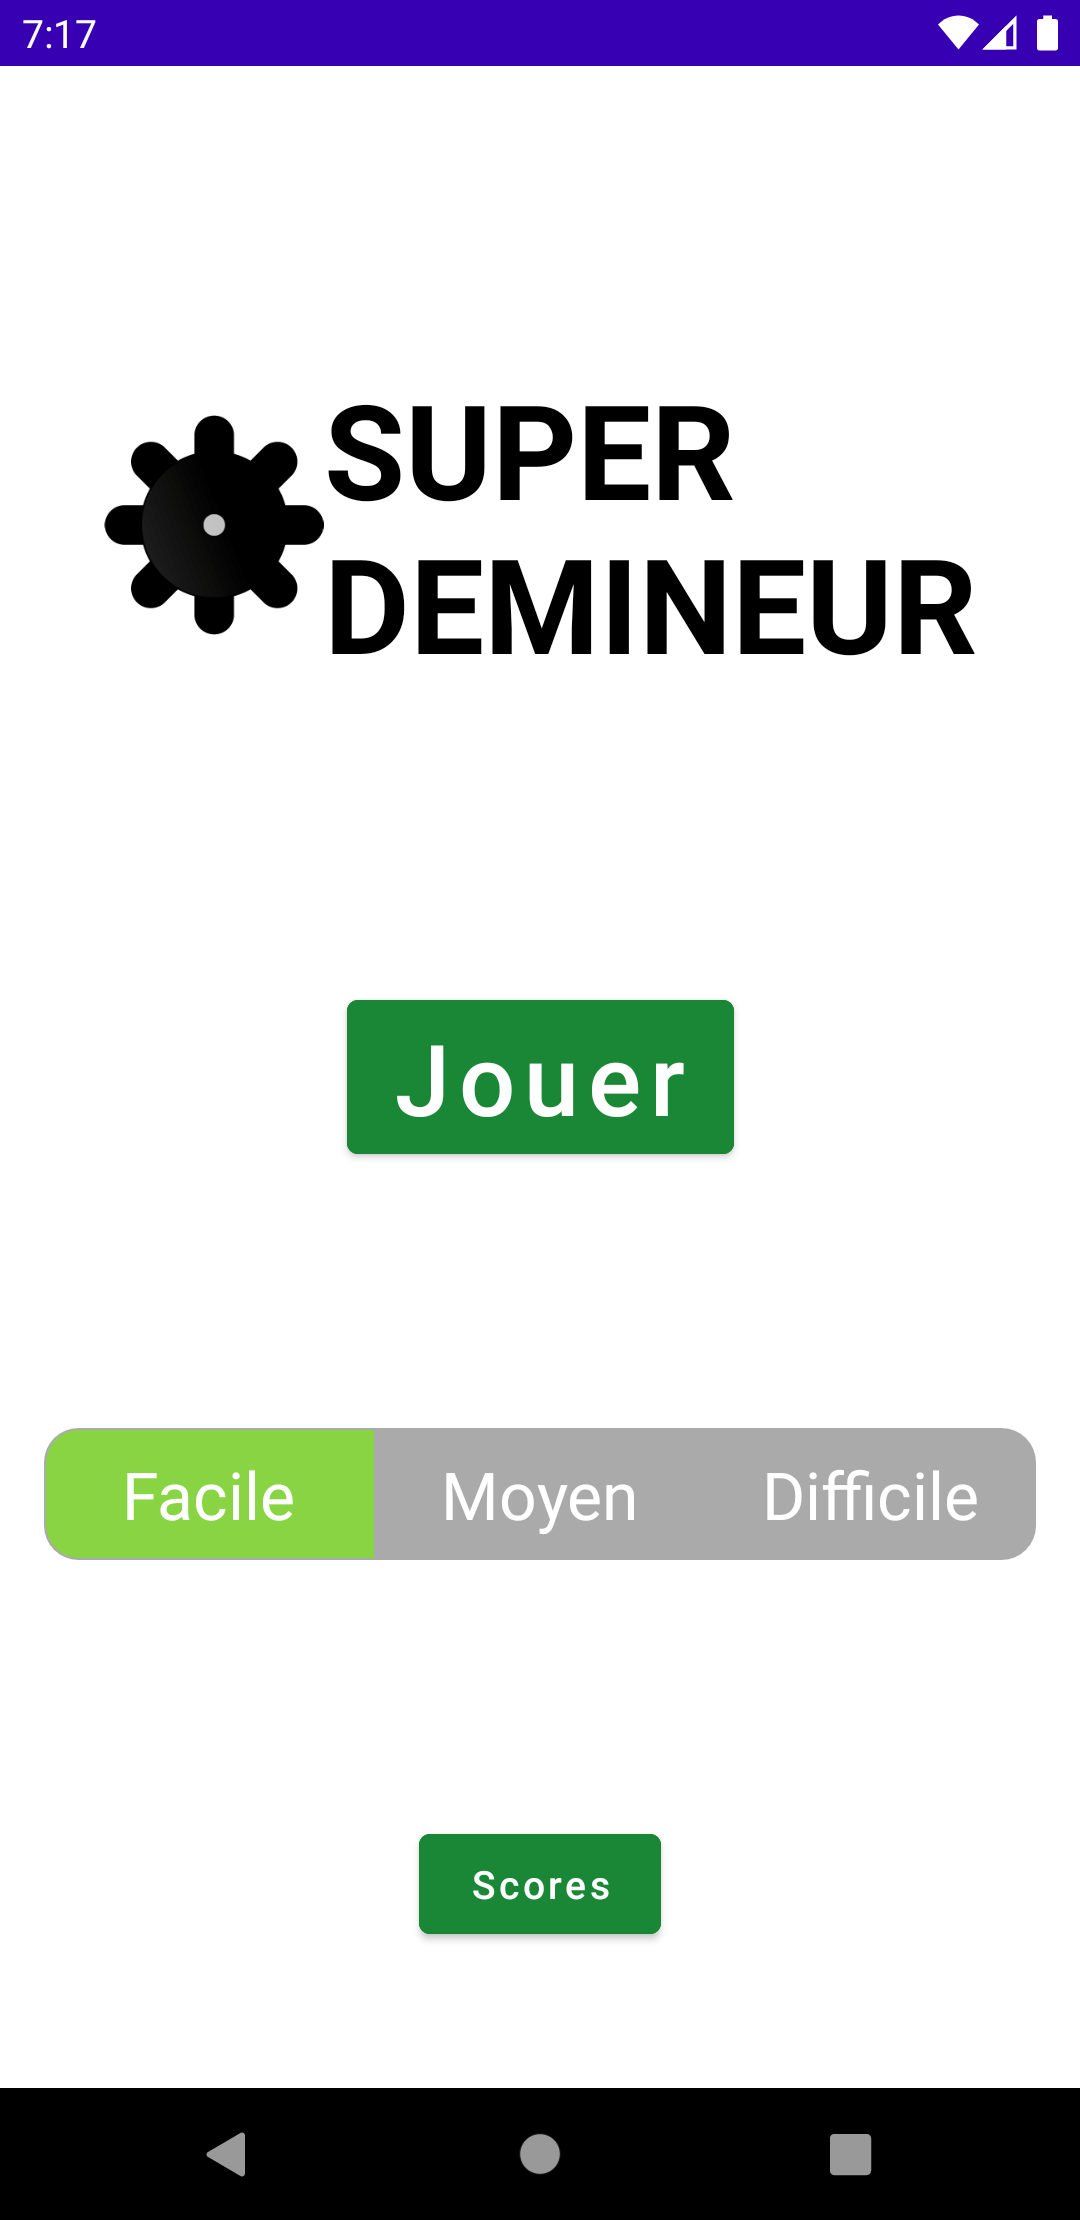
\includegraphics[width=0.33\linewidth]{androidSegmented.png}
    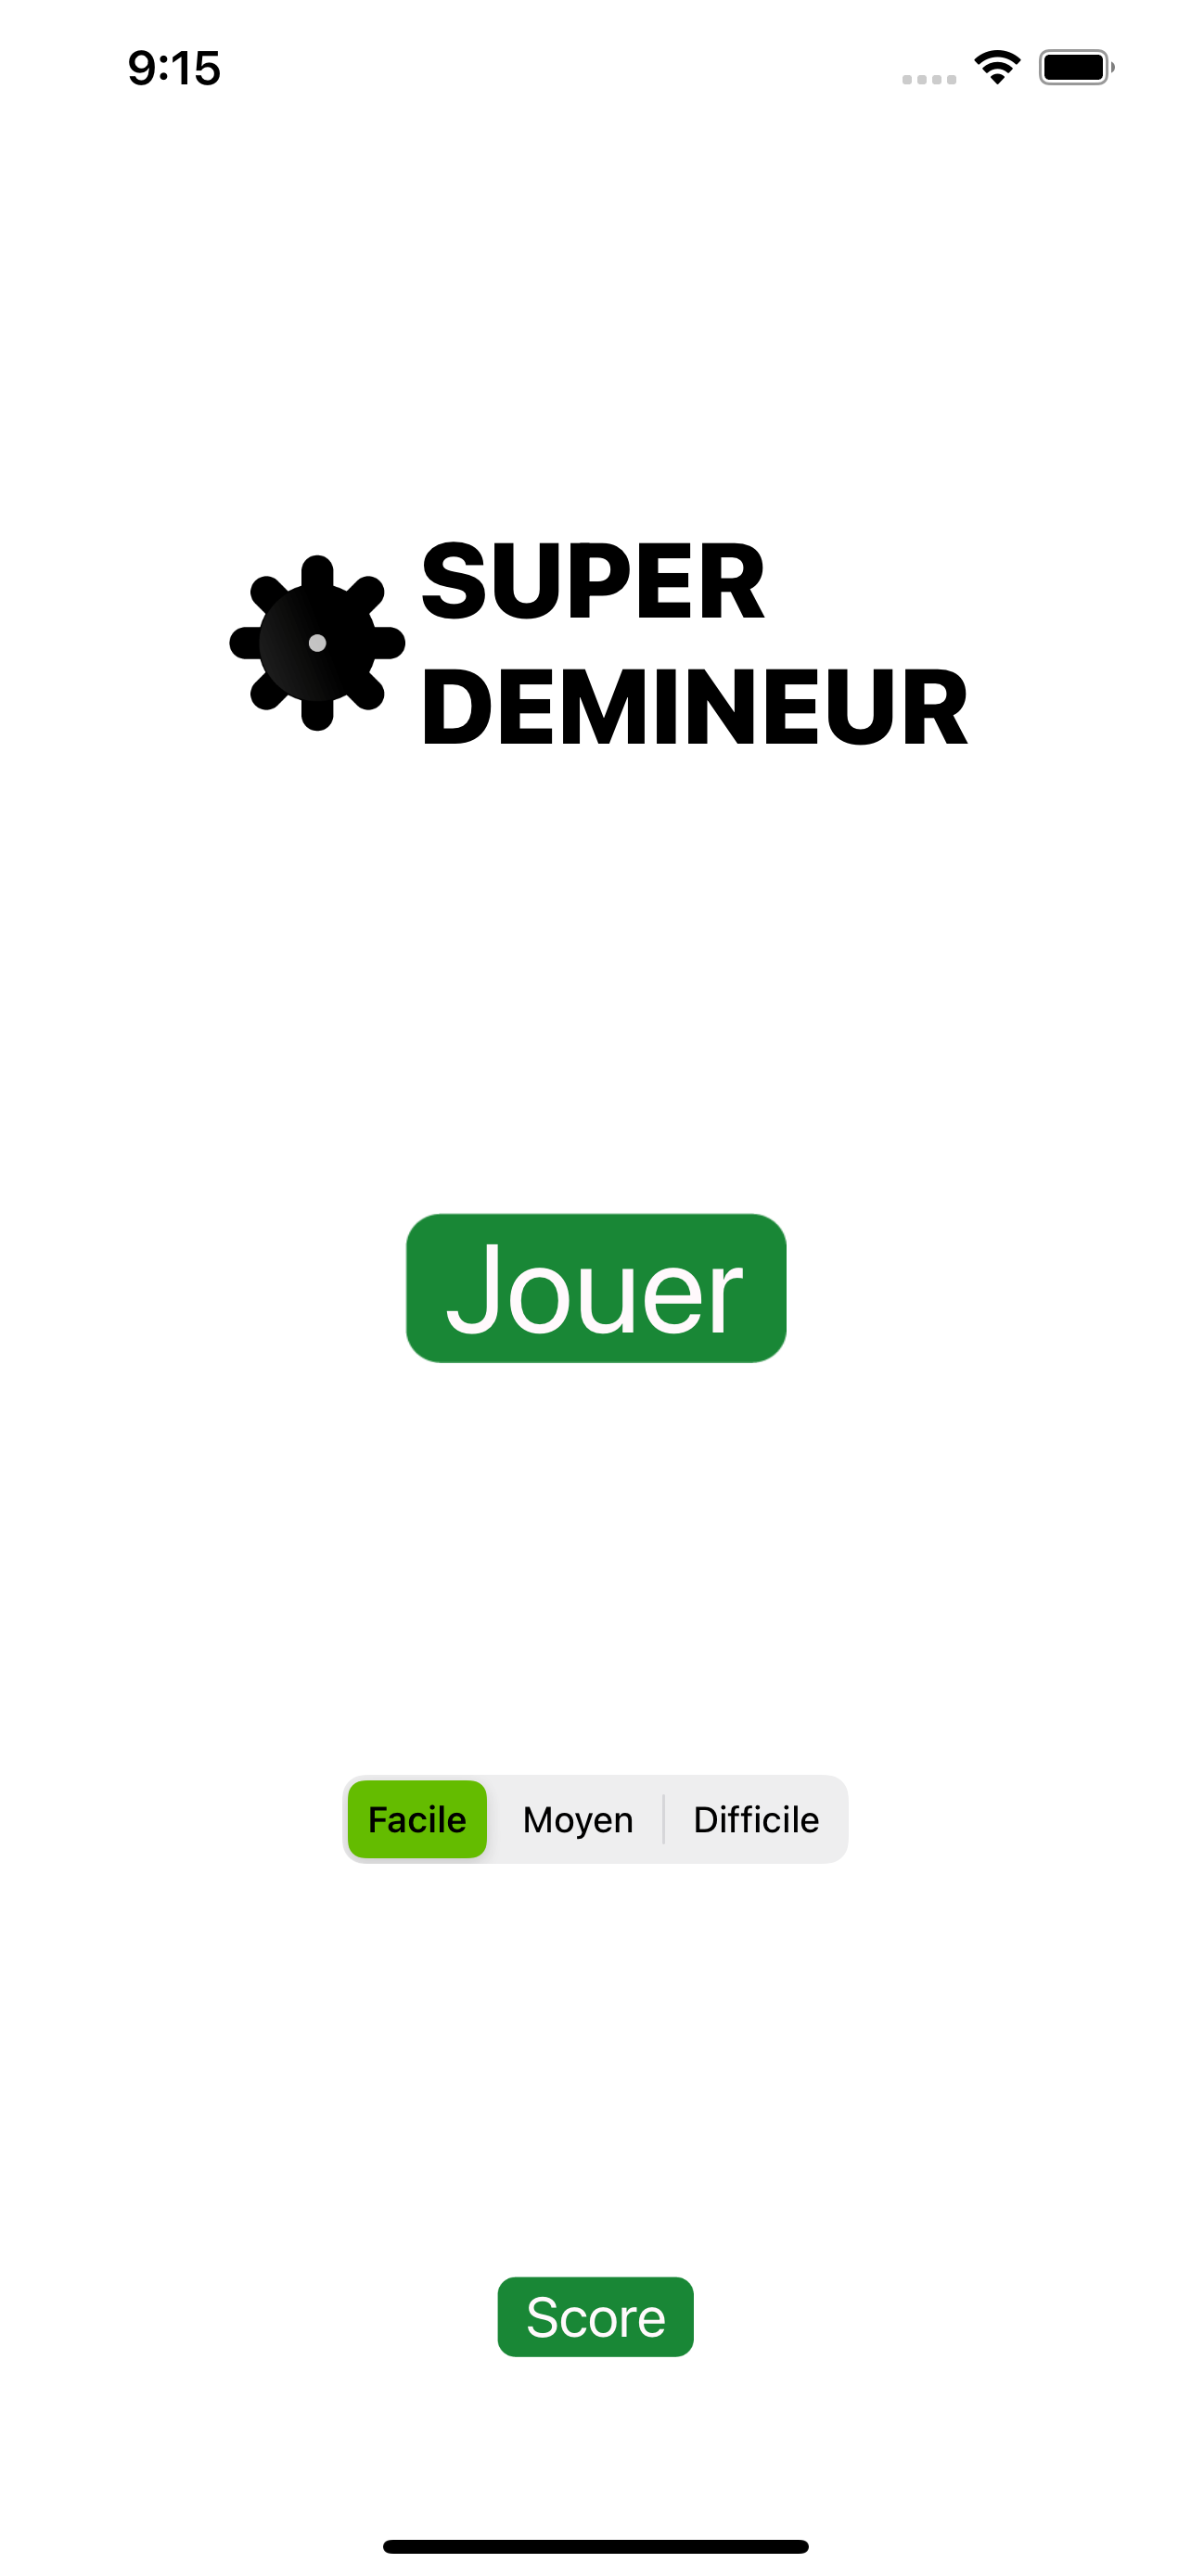
\includegraphics[width=0.33\linewidth]{MainView_iOs.png}
    \caption{ RadioGRoup pour Android à gauche et SegmentedButton pour iOs à droite}
\end{figure}


\section{iOs}

Dans cette section nous détaillerons les choix de développement de la version iOs du Super Démineur. 

\subsection{Représentation de la grille}

Sous iOs, la grille du jeu a été générée dynamiquement sans contraintes à l'aide de boutons qui s'adaptent à toutes les tailles d'écran et à toute orientation. \\\\
La grille a été représentée sous forme de bouton car n'ayant aucune contraintes de layout il été donc préférable d'avoir le clique du joueur corrélé avec la case via la callback du bouton. 
Ainsi chaque bouton, représenté par une case, est instancié à une position et une dimension donnée puis ajouté à la BattleView afin de former la grille de jeu.\\

\noindent \underline{\textit{Constructeur de la classe Case:}}
\begin{minted}[frame=lines,framesep=10pt]{swift}
//Initialisation du bouton
self.caseBtn = UIButton(frame: CGRect(x: xPos, y: yPos, width: dim, height: dim)) 

//Ajout de la case dans la vue
grille.addSubview(caseBtn)
\end{minted}


\subsubsection{La position des boutons}

Dans le but de centrer la grille du jeu, on applique le même décalage à toute les positions des boutons de la grille par rapport au dimension de l'écran.\\

\noindent \underline{\textit{Calcul de la position des boutons :}}\\
Soit $W,H$ respectivement la largeur et la hauteur de l'écran. \\
Soit $l,c$ respectivement le nombre de ligne et le nombre de colonne de la grille. \\
Soit $i,j$ les coordonnées  des boutons dans la grille. \\
Soit $d$ les dimensions des boutons dans la grille. \\

\noindent Alors la position $(x,y)$ en absolue dans la BattleView d'un bouton de coordonnée $(i,j)$ est donnée par :\\

$$
\left\{
    \begin{array}{ll}
        x=i\times d+\frac{(W-l\times d)}{2} \\
        y=j\times d+\frac{(H-c\times d)}{2}
    \end{array}
\right.
$$

\subsubsection{La dimension des boutons}

Afin que la grille du jeu soit adapté a toute les tailles d'écran, il fallait dimensionner les boutons en conséquence. Ainsi, nous avons décidé que la dimension des cases serait arbitrairement ajusté par rapport à la plus grande longueur de l'écran, à savoir sa hauteur.\\

\noindent \underline{\textit{Calcul de la dimension des boutons :}}\\
Soit $H$ la hauteur de l'écran.\\
Soit $m$ le \% de l'écran de la marge désirée entre le grille de jeu et l'écran (dans le sens de la hauteur).\\
Soit $l$  le nombre de ligne.\\

\noindent Alors la dimension $d$ des boutons est donnée par : 
$$d = \frac {(1 - m)\times W }{l}$$


\subsubsection{L'orientation des boutons}

L'application pouvant être joué aussi bien horizontalement que verticalement et la grille de jeu n'étant soumise à aucune contrainte, il était donc nécessaire d'ajuster dynamiquement la position des boutons en réponse à la rotation de l'écran. \\

A chaque rotation de l'écran, la fonction ViewWillTransition du contrôleur de la BattleView s'éxécute. Ainsi si l'on souhaite réaliser des actions suivant la rotation de l'écran, il suffit de surcharger cette fonction. \\


\noindent \underline{\textit{Surcharge de la fonction ViewWillTransition}}

\begin{minted}[frame=lines,framesep=10pt]{swift}
//Appel du constructeur de la superClass
super.viewWillTransition(to: size, with: coordinator)

//Redessinage de la grille en fonction de l'orientation de destination de l'écran
gridView.DrawGrid(heightScreenDestination: size.height,widthScreenDest: size.width)
\end{minted}


\paragraph{\underline{Remarque:}} Pour chaque case, la position des boutons sera changé en fonction de hauteur et la largeur de l'écran. Ceci sera réalisé en inversant les lignes des colonnes et en inversant également les décalages en ligne et en colonne (ci-dessous $shift_{x}$ et $shift_{y}$). \\

\noindent \underline{\textit{Transposition des cases}}
\begin{minted}[frame=lines,framesep=10pt]{swift}
//Mode paysage
if(widthScreenDest > heightScreenDestination)
{
    self.grille[i][j].setPos(posX:(j*caseDimension+Int(shift_x)), 
    posY: (i*self.caseDimension+Int(shift_y)))
}
else //Move portrait
{
    self.grille[i][j].setPos(posX:(i*caseDimension+Int(shift_y)), 
    posY: (j*self.caseDimension+Int(shift_x)))
}
\end{minted}

\paragraph{\underline{Remarque:}} Seule la grille a été représenté dynamiquement sans contrainte, tous les autres éléments de l'interface ont été placé à l'aide de contrainte en \%  de l'écran dans le storyboard. \\



\subsection{Passage d'information entre les vues avec les segues}

Les trois vues présenté précédemment ont chacune leurs ViewController : 
\begin{itemize}
    \item  BattleViewController, le contrôleur de la scène de jeu
    \item  ScoreViewController, le contrôleur de la scène des scores
    \item  MainViewController, le contrôleur de la scène principale\\
\end{itemize}

Afin de passer des informations entres les différents contrôleurs, on utilisera les segues suivants :
\begin{itemize}
    \item  BackToMain : ramène les performances du joueur dans le tableau des scores dans la vue principale
    \item  ShowScore : transfert de la MainView à la ScoreView le tableau des scores de la vue prinpale
    \item  StartABattle : transfert la valeur de difficulté choisis par l'utilisateur dans la fenêtre principale 
\end{itemize}

\begin{figure}[H]
    \centering
        \begin{tikzpicture}
        \sbEntree{E}
        \sbBlocr{r1}{BattleViewController}{E}
        \sbBlocr[7]{r2}{MainViewController}{r1}
        \sbBlocr[5]{r3}{ScoreViewController}{r2}
        \sbRelier[BackToMain]{r1}{r2}
        \sbRelier[StartABattle]{r2}{r1}
        \sbRelier[ShowScore]{r2}{r3}
        \end{tikzpicture}
        \caption{Diagramme des vues et segues associés}
\end{figure}


Concrètement chaque contrôleur de départ du segue surcharge la méthode "prepare" pour, comme son nom l'indique, préparer le contexte du contrôleur d'arrivé.\\ 
Par exemple pour le segue de BackToMain ceci s'est réalisé en deux étapes : 
\begin{itemize}
    \item  Le cast du contrôleur de destination en MainViewController
    \item  Puis l'ajout de la performance du joueur à la MainViewController en utilisant ses propres méthodes \\
\end{itemize}
 
\noindent \underline{\textit{\cite{devLibreSegue}Configuration du Segue BackToMain dans BattleViewController}}
\begin{minted}[frame=lines,framesep=10pt]{swift}
override func prepare(for segue: UIStoryboardSegue, sender: Any?) 
{
    if segue.identifier == "BackToMain"
    {
        let VCDestination = segue.destination as! MainViewController
                    
        //Puis on ajoute la scoreDifficultyList dans le MainVC
        VCDestination.addToScoreDifficultyList(scoreDifficultyList: self.scoreDifficultyList)
    }
}
\end{minted}


\subsection{Présentation sous forme de liste avec la UITableView}

Dans la vue des scores on présentera sous forme de liste un tableau à 2 dimensions $dataTabView$ (importé par la suite dans la vue des scores par le segue ShowScore) dont la première représente les sections de la liste et la deuxième les informations dans les cellules des sections. 

\paragraph{\underline{Exemple:}} le tableau des données à représenter dans la liste des scores est sous la forme : $$[[Score_{Facile},Temps_{Facile}, Date_{Facile}], [Score_{Moyen},Temps_{Moyen}, Date_{Moyen}]]$$
où $Score_{Facile}$ est le score du joueur en \% dans le mode facile du jeu, $Temps_{Facile}$ le 
temps mis par le joueur pour réaliser cette performance et enfin $Date_{Facile}$ la date a laquelle il l'a réalisé. 

\subsubsection{Implémentation du délégate}

Dans un premier temps le contrôleur de la vue des scores implétementera deux délégates :  UITableViewDelegate et UITableViewDataSource. Suite à cela on crée un lien @IBOutlet entre la UITableView et le contrôleur pour finaliser l'implémentation de la delegate dans la méthode ViewDidLoad. \cite{iosProf} \\

\noindent \underline{\textit{ViewDidLoad de ScoreViewController}}
\begin{minted}[frame=lines,framesep=10pt]{swift}
class ScoreViewController: UIViewController ,  UITableViewDelegate , 
UITableViewDataSource{

@IBOutlet weak var myScoreTableView: UITableView!

override func viewDidLoad()
{
    super.viewDidLoad()
    
    //Implémentation delegate
    myScoreTableView.dataSource = self
    myScoreTableView.delegate = self
}
\end{minted}

\subsubsection{Implémentation des UITableViewCell}

La UITableView est composé de UITableViewCell dont on architecture le visuel dans le storyboard et la class grâce à des attributs @IBOutlet. De plus, on ajoutera également une fonction $setScoreTimeDate()$ pour mettre en forme les labels de la cellule.\\


\noindent \underline{\textit{Class de UITableViewCell}}
\begin{minted}[frame=lines,framesep=10pt]{swift}
class ScoreCell: UITableViewCell  {
    
@IBOutlet weak var DateLabel: UILabel! //Lien vers le label de la date dans la cellule
@IBOutlet weak var TimeLabel: UILabel! //Lien vers le label du temps dans la cellule
@IBOutlet weak var ScoreLabel: UILabel! //Lien vers le label du score dans la cellule

//Formattage des données 
public func setScoreTimeDate(score : Int, time: Int, date:Date)
{
    self.ScoreLabel.text = String(score) + "%"
    self.TimeLabel.text = String(format: "%02d:%02d", time/60, time%60)
    self.DateLabel.text = date.getFormattedDate(format: "yyyy-MM-dd")
}}
\end{minted}

\subsubsection{Configuration du delegate}

Puis on configure les fonctions du delegate en accord avec l'architecture de  $dataTabView$ présenté précédemment. Plus précisément on aura : 
\begin{itemize}
    \item  autant de section que dans la première dimension du tableau, donc la fonction numberOfSections retournera $dataTabView.count$
    \item  autant de d'élément dans une section donnée qu'il y a d'élément dans la deuxième dimension du tableau, donc la fonction doté de l'argument numberOfRowsInSection retournera $dataTabView[section].count$
    \item  les données de $dataTabView$ qui seront ajouté dans la cellule via $setScoreTimeDate()$\\
\end{itemize}

\noindent \underline{\textit{Quelques fonctions du delegate}}
\begin{minted}[frame=lines,framesep=10pt]{swift}

//Configuration du nombre de section
func numberOfSections(in tableView: UITableView) -> Int {return dataTabView.count}

//Configuration du nombre d'élément dans la section
func tableView(_ tableView: UITableView, numberOfRowsInSection section: Int) -> Int 
{
    return dataTabView[section].count
}

//Configuration des élements du tableau
func tableView(_ tableView: UITableView, cellForRowAt indexPath: IndexPath) 
-> UITableViewCell
{
    //On récupère la cellule du tableau
    let cell = tableView.dequeueReusableCell(withIdentifier: "scoreCell") as! ScoreCell
    
    //Dans laquelle on ajoute les éléments de dataTabView
    cell.setScoreTimeDate(score: dataTabView[indexPath.section][indexPath.row].0, 
    time: dataTabView[indexPath.section][indexPath.row].1, 
    date: dataTabView[indexPath.section][indexPath.row].2)
    
    return cell
}
\end{minted}


\subsection{Persistance des données avec UserDefaults}


\subsubsection{Sauvegarde des données}

Pour notre application nous souhaitions réaliser une sauvegarde de la progression du joueur. Cela revient donc à sauvegarder le tableau des scores $scoreDifficultyList$ présents dans la vue principale (qui est ensuite importé par le segue ShowScore dans la vue des scores). \\

On effectue cette sauvegarde avec la fonction $UserDefaults.standard.set()$ précédé d'une sérialisation des données de $scoreDifficultyList$ car cette fonction ne permet pas la sauvegarde de ce tableau tel qu'il est architecturé :
$$[(Score,Difficulty,Time,Date)]$$

Ainsi nous réalisons donc un découpage des données de $scoreDifficultyList$ en sous-tableau de manière à les formater pour la sauvegarde à chaque fois qu'une donnée est ajouté en provenance de la BattleView.\\


\noindent \underline{\textit{Sérialisation et sauvegarde des données}}
\begin{minted}[frame=lines,framesep=10pt]{swift}
 func addToScoreDifficultyList(scoreDifficultyList :[(Int,Int,Int)])
{
//On initialise des tableaux d'entiers/date
var date_serie : [Date] = []
var score_serie : [Int] = []
var temps_serie : [Int] = []
var difficulte_serie : [Int] = []

//Ajout des données en provenance de la BattleView
for (score,difficulty,temps) in scoreDifficultyList
{
    date_serie.append(Date())
    score_serie.append(score)
    temps_serie.append(temps)
    difficulte_serie.append(difficulty)
}

//Ajout des données déjà existante dans la MainView
for (score,difficulty,temps, date) in MainViewController.scoreDifficultyList
{
    date_serie.append(date)
    score_serie.append(score)
    temps_serie.append(temps)
    difficulte_serie.append(difficulty)
}

// Enfin on sauvegarde l'ensemble des données de l'utilisateur dans UserDefaults
UserDefaults.standard.set(date_serie, forKey: "date")
UserDefaults.standard.set(score_serie, forKey: "score")
UserDefaults.standard.set(temps_serie, forKey: "temps")
UserDefaults.standard.set(difficulte_serie, forKey: "difficulte")
}
\end{minted}

\subsubsection{Restauration des données}

Au lancement de l'application la vue principale est chargée et les valeurs stockés dans $UserDefaults.standard$ y sont toujours car persistante. Ainsi il suffit de récupérer les données et de les dé-sérialiser pour remplir notre tableau des scores $scoreDifficultyList$.\\

\noindent \underline{\textit{Désérialisation et restauration des données}}
\begin{minted}[frame=lines,framesep=10pt]{swift}

//Déserialisations des données
let difficulte_serie = UserDefaults.standard.object(forKey: "difficulte") as? [Int] ?? []
let date_serie = UserDefaults.standard.object(forKey: "date") as? [Date] ?? []
let temps_serie = UserDefaults.standard.object(forKey: "temps") as? [Int] ?? []
let score_serie = UserDefaults.standard.object(forKey: "score") as? [Int] ?? []

//Si une donnée a déjà été sauvegardé
if(!difficulte_serie.isEmpty)
{
    //Alors on l'a restitue dans le tableau des scores
    for i in 0...difficulte_serie.count-1
    {
        MainViewController.scoreDifficultyList.append((score_serie[i],difficulte_serie[i],
        temps_serie[i],date_serie[i]))
    }
}
\end{minted}



\section{Android}
Dans cette section nous détaillerons les choix de développement de la version Android du Super Démineur.

\subsection{Représentation de la grille}

Contrairement à la version iOs, la version Android utilise une vue custom \cite{androidProf} pour  afficher le jeu et non des boutons. Ce choix est dû à l' API  de layout assez capricieux, ce qui rendait le positionnement en absolu des boutons difficile.\\

La grille possède un tableau à deux dimensions de Cases, les Objets "Cases" ne servent qu'à faciliter l'affichage et l'algorithme de creusage récursif. Par exemple, pour afficher un drapeau sur la case, il faut dessiner le drawable sur le canvas et donc gérer soit même le ratio et le centrage de l'image:\\

\noindent\underline{\textit{drawImg de la  classe Case:}}
\begin{minted}[frame=lines,framesep=10pt]{java}
// Dessine une image au centre de la case, où un scale de 1 vaut taille, 
// tout en conservant le ratio
private void drawImg(Canvas canvas, Drawable img, float scale){
    int imgWidth = img.getIntrinsicWidth();
    int imgHeight = img.getIntrinsicHeight();
    float targetWidth, targetHeight;
    // On conserve le ratio de l'image
    if(imgWidth < imgHeight){
        float ratio = (float) imgWidth/(float)imgHeight;
        targetWidth = taille*scale*ratio;
        targetHeight = taille*scale;
    } else {
        float ratio = (float )imgHeight/ (float) imgHeight;
        targetWidth = taille*scale;
        targetHeight = taille*scale*ratio;
    }
    // Décalage pour centrer l'image
    float xOffset = (taille-targetWidth) / 2.0f;
    float yOffset = (taille-targetHeight) / 2.0f;
    // Repositionnement et redimensionnement de l'image
    img.setBounds((int) (x+xOffset), 
                  (int) (y+yOffset), 
                  (int) (x+xOffset+targetWidth), 
                  (int)(y+yOffset+targetHeight));
    img.draw(canvas);
    }
\end{minted}

\subsubsection{La position des cases}

La vue Grille, prend tout l'espace disponible déterminée par  les contraintes de l'activité Partie, or les cases sont carrés, il faut donc centrer le dessin du plateau dans le canvas.\\

\noindent Soit $W,H$ la largeur et la hauteur de la vue, déterminées par le ConstraintLayout de l'activité Partie.\\
Soit $n,m$ le nombre de lignes et le nombre de colonnes déterminés à l'initialisation de la Grille.\\
Soit $d$ la dimension des cases que l'on déterminera plus-tard.\\
Pour tout $(i,j)\in [\![0, n-1]\!]\times [\![0, m-1]\!]$, on note $(x,y)\in [0, W]\times [0, H]$ la coordonnée de la case $c_{i,j}$ dans le canvas.\\

\noindent En fonction de l'orientation on transpose le tableau de cases, on distinguera donc le cas paysage du cas portrait :\\

\noindent On pose 
$$dx = \begin{dcases}
    \frac{W-m\times d}{2} \text{ si mode portrait} \\
    \frac{W-n\times d}{2} \text{ si mode paysage}
\end{dcases} \text{ et } dy = \begin{dcases}
    \frac{H-n\times d}{2} \text{ si mode portrait} \\
    \frac{H-m\times d}{2} \text{ si mode paysage}
\end{dcases}$$ 

le décalage en $x$ et en $y$ par rapport  à l'origine du canvas (coin supérieur gauche). On a donc : \\

$$(x,y) = \begin{dcases}
    \left( dx+j\times d, dy+i\times d\right) \text{ si mode portrait} \\
    \left( dx+i\times d, dy+j\times d\right) \text{ si mode paysage}
\end{dcases}$$



\subsubsection{La dimension des cases}
\noindent Soit $W,H$ la largeur et la hauteur de la vue, déterminées par le ConstraintLayout de l'activité Partie.\\
Soit $n,m$ le nombre de lignes et le nombre de colonnes déterminés à l'initialisation de la Grille.\\
On note $d$ la dimension des cases.\\

\noindent En fonction de l'orientation on transpose le tableau de cases, on distinguera donc le cas paysage du cas portrait.\\

$$d=\begin{dcases}
\Min{}\left(\frac{W}{m}, \frac{H}{n}\right) \text{ si mode portrait} \\
\Min{}\left(\frac{W}{n}, \frac{H}{m}\right) \text{ si mode paysage}
\end{dcases}$$

\subsubsection{Gestion des inputs}
La classe grille doit aussi gérer la position du clique de l'utilisateur pour déterminer la case pressée.\\

\noindent Soit $(x,y)$ les coordonnées du clique dans la vue Grille.\\
Soit $d$ la taille des cases.\\
Soit $dx$ (resp $dy$) le décalage en $x$ (resp $y$) pour centrer les cases dans la vue.\\
On détermine les coordonnées $(i,j)$ dans le tableau de la case pressée comme suit:\\

$$ (i,j) = \begin{dcases}
    \left(\left\lfloor\frac{x - dx}{d}\right\rfloor, \left\lfloor\frac{y - dy}{d}\right\rfloor \right) \textit{ si mode portrait}\\
     \left(\left\lfloor\frac{y - dy}{d}\right\rfloor, \left\lfloor\frac{x - dx}{d}\right\rfloor \right) \textit{ si mode paysage}
\end{dcases}$$

Bien entendu, si $(x < dx)\vee (x > dx+d\times m) \vee (y < dy) \vee (y > dy+d\times n)$ est vraie avec $n$ le nombre de lignes et $m$ le nombre de colonnes, alors on ignore le clique puisqu'il n'est pas dans la zone où sont dessinées les cases.\\

\noindent \underline{\textit{onTouchEvent}}

\begin{minted}[frame=lines,framesep=10pt]{java}
// Coordonnées du pointeur
float mx = event.getX();
float my = event.getY();
// En mode landscape (rotation != 0) on prend la transposée de la grille
// c'est à dire on inverse n et m
int rotation = display.getRotation();
int tm = Surface.ROTATION_0 != rotation ? n : m;
int tn = Surface.ROTATION_0 != rotation ? m : n;
// Le pointeur doit être dans la zone de dessin de la grille si non on ne fait rien
if(mx < xOffset || mx > xOffset+tailleCase*tm || my < yOffset || my > yOffset+tailleCase*tn)
    return true;
// On recup les coordonnées de la case dans la grille en fonction de la rotation
// En mode landscape (rotation != 0) on prend la transposée
int j = (int) ((mx - xOffset) / tailleCase);
int i = (int) ((my - yOffset) / tailleCase);
// On permute i et j si besoin
if(Surface.ROTATION_0 != rotation){ int tmp=i; i=j; j=tmp;}
...
\end{minted}

\subsection{Passage d'information entre les vues}
Les trois vues présentées \hyperref[fig:figure1]{\textcolor{blue}{\underline{précédemment}}} ont chacune leurs activités : 
\begin{itemize}
    \item  ScoresActivity, l'historique des scores
    \item  MainActivity, le menu principal
    \item  PartieActivity, le jeu \\
\end{itemize}

Afin de passer des informations entres les différentes activités, on utilise le système d'intent d'Android. 

\begin{figure}[H]
    \centering
        \begin{tikzpicture}
        \sbEntree{E}
        \sbBlocr{r1}{PartieActivity}{E}
        \sbBlocr[7]{r2}{MainActivity}{r1}
        \sbBlocr[7]{r3}{ScoresActivity}{r2}
        \sbRelier[jouer]{r2}{r1}
        \sbRelier[voirScores]{r2}{r3}
        \end{tikzpicture}
        \caption{Diagramme des Activités et des intents associés}
\end{figure}

En revanche, la structure de données qui continent l'historique des scores n'est pas transmise à l'activité Partie, elle est directement accessible en temps que champ publique statique:\\

\noindent \underline{\textit{MainActivity: structure de données des scores}}
\label{code:listdata}
\begin{minted}[frame=lines,framesep=10pt]{java}
// Static pour faciliter l'ajout de données depuis l'activité PartieActivity
public static ArrayList<String> stats = new ArrayList<>();
}
\end{minted}
Il en a été décidé ainsi pour faciliter le stockage des données critiques en mémoire à chaque fin de partie.\\

Hormis l'ajout des statistiques à chaque fin de partie, seule l'activité Main a besoin d'envoyer des informations : c'est elle qui indique à la partie le niveau de difficulté choisi par l'utilisateur. De même, c'est elle qui donne l'historique des statistiques des parties à l'activité Scores, qui ne sert qu'à les afficher.\\

\noindent \underline{\textit{MainActivity: jouer() et voirScore()}}

\begin{minted}[frame=lines,framesep=10pt]{java}
// Lance l'activité du jeu avec le bon niveau de difficulté
public void jouer(View v){
    Intent intent = new Intent(this, PartieActivity.class);
    // On recup la difficuté choisie
    int radioID = levelSelector.getCheckedRadioButtonId();
    RadioButton radioLevel = findViewById(radioID);
    int level = Integer.parseInt(radioLevel.getTag().toString());
    intent.putExtra("level", level);
    startActivity(intent); // On lance PartieActivity
}
// Lance l'activité de l'historique des scores
public void voirScores(View v){
    Intent intent = new Intent(this, ScoresActivity.class);
    intent.putStringArrayListExtra("array", stats); // On lui donne les données
    startActivity(intent); // On lance ScoresActivity
}
\end{minted}

\noindent\underline{\textit{Exemple de récupération des données via un intent :}}
\begin{minted}[frame=lines,framesep=10pt]{java}
...
// On recup les stats depuis la vue principale
Intent intent = getIntent();
stats = intent.getStringArrayListExtra("array");
...
\end{minted}


\subsection{Présentation sous forme de liste avec ExpandableListView}

Comme \hyperref[code:listdata]{\textcolor{blue}{\underline{indiqué plus haut}}}, l'historique des statistiques de chaque parties est représenté par une liste de chaînes de caractères. L'avantage d'une ExpandableListView est qu'il est possible de trier les cellules par catégories, de plus, les catégories peuvent afficher et cacher leur liste de façon dynamique. Nous avons opté pour 3 catégories liées au niveau de difficulté : Facile, Moyen et Difficile.

\begin{figure}[H]
    \centering
    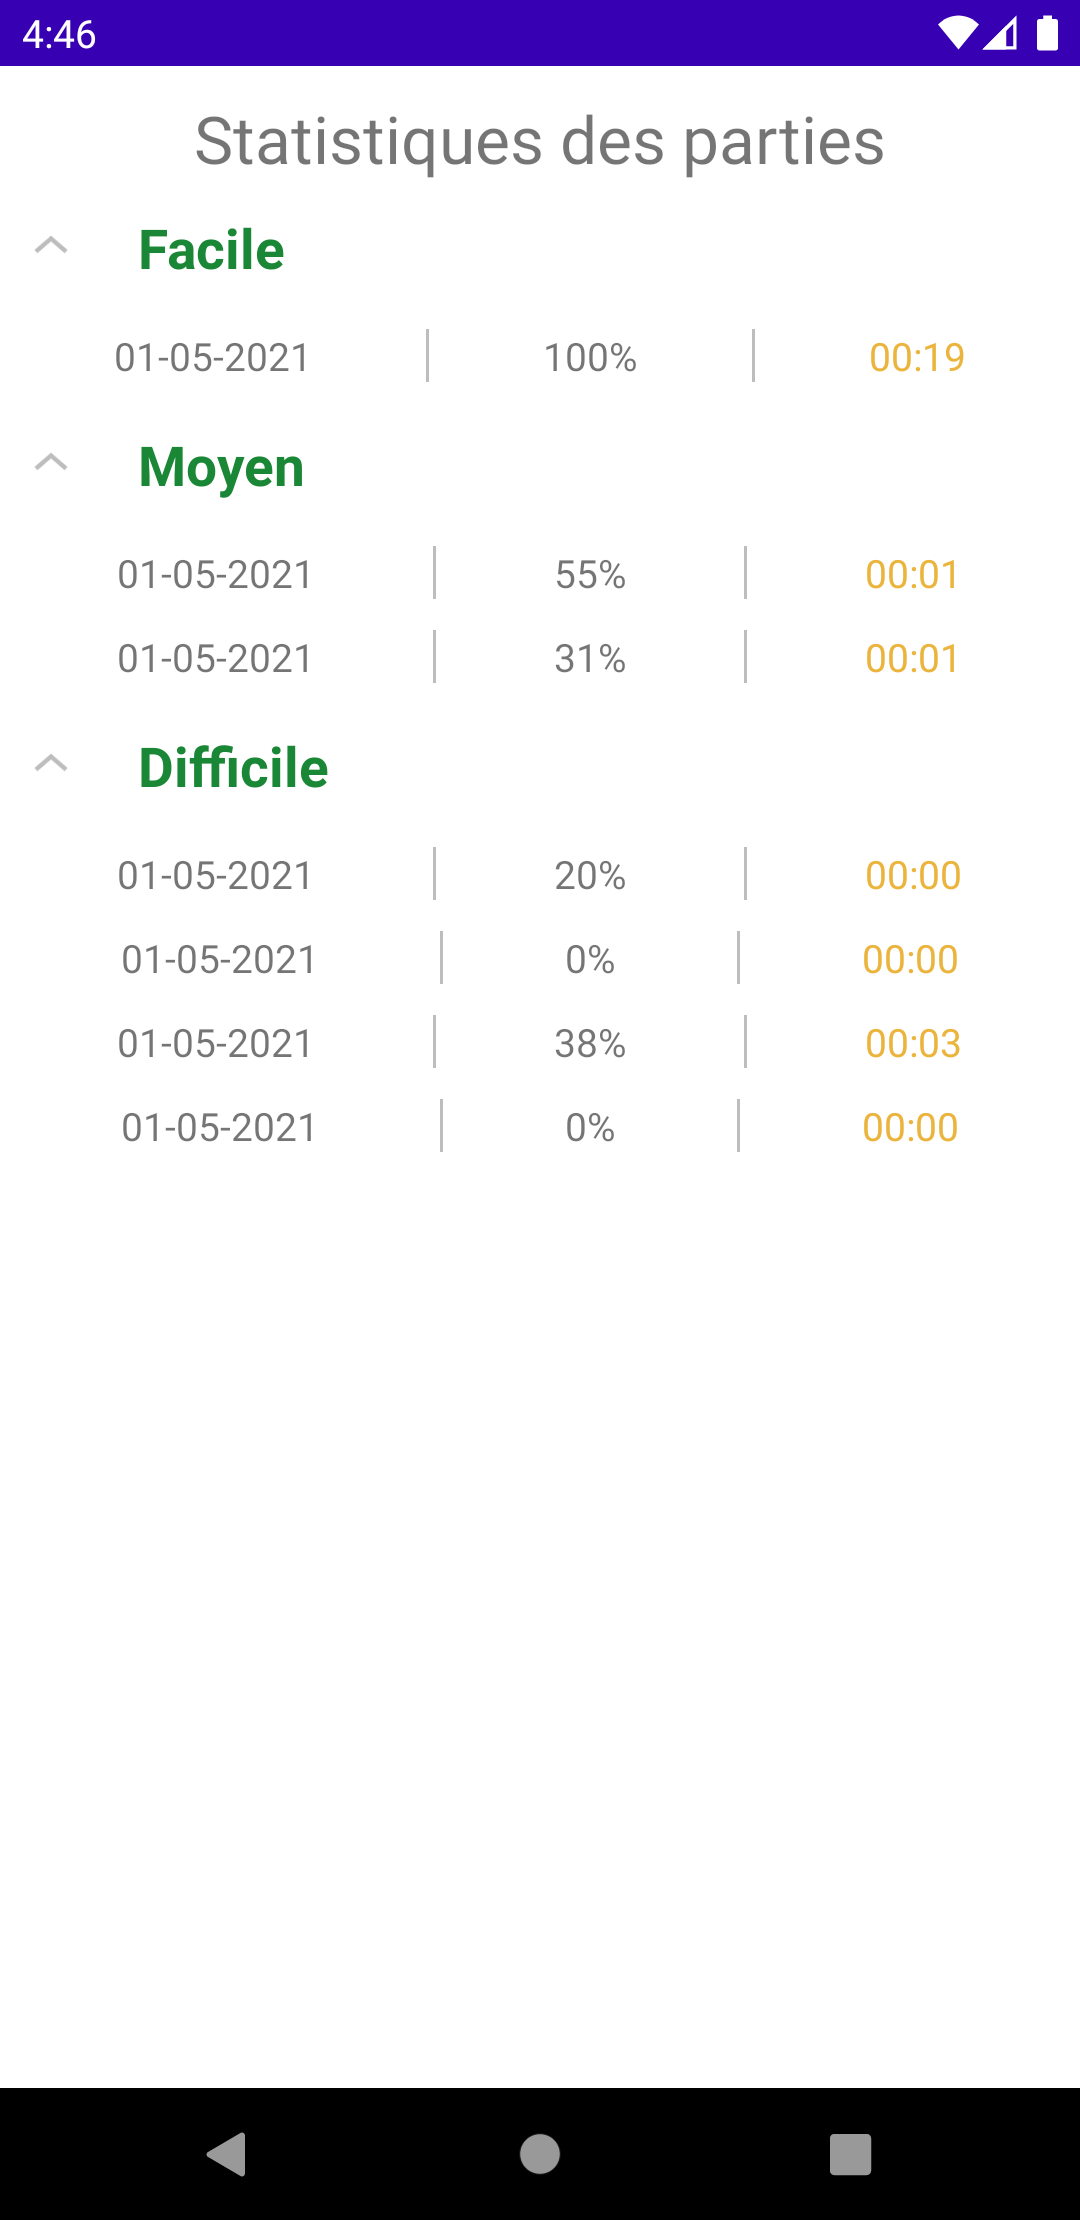
\includegraphics[width=0.3\linewidth]{androidListView.png}
    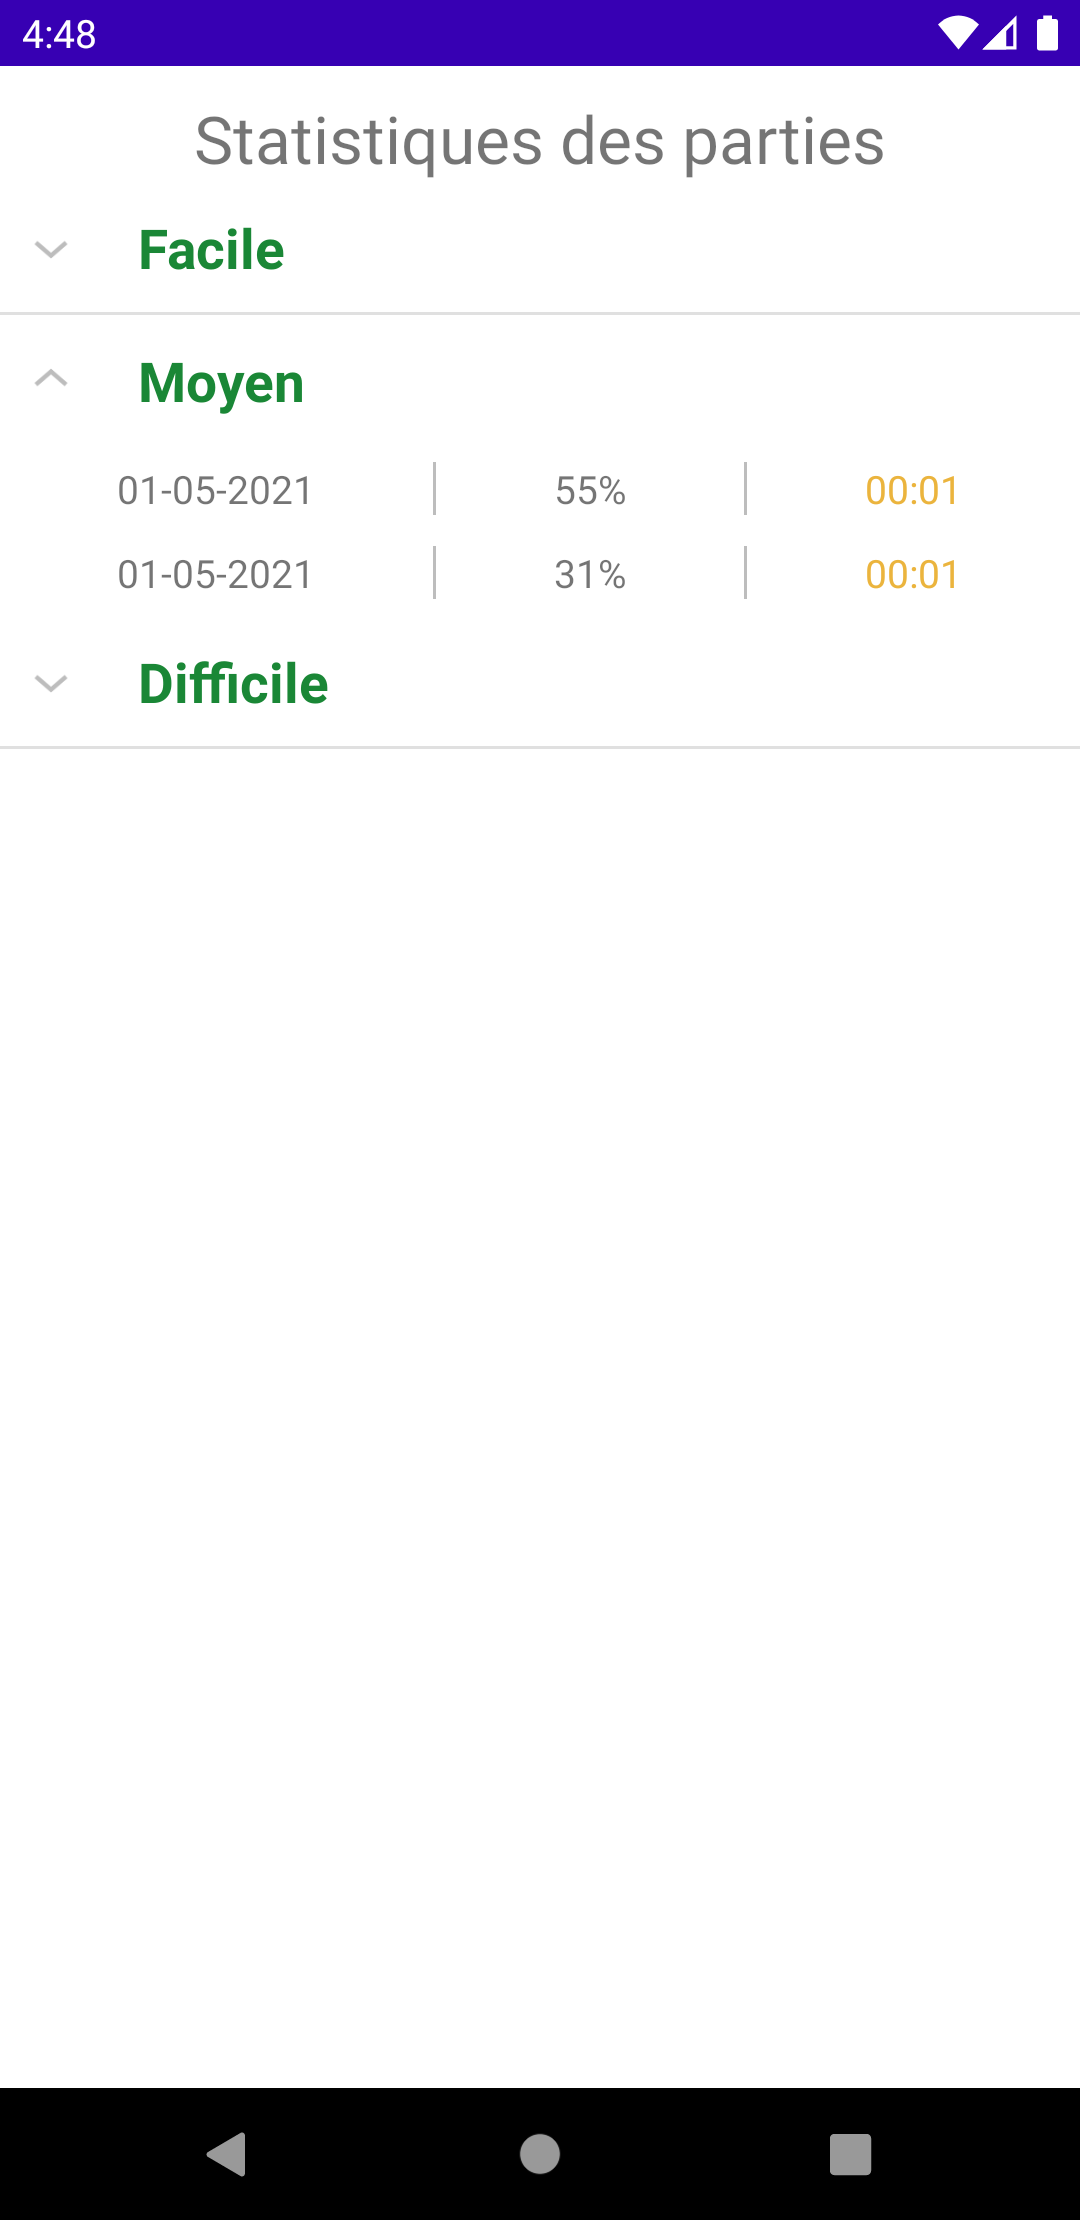
\includegraphics[width=0.3\linewidth]{androidListView2.png}
    \caption{ScoresActivity}
\end{figure}

\subsubsection{Représentation des données}
\label{section:dataformat}
les statistiques d'une partie sont stockées dans une seule chaîne de caractère suivant ce format:\\

\begin{center}
    \textit{date;score;temps;difficulté}
\end{center}

Avec pour conventions:
\begin{itemize}
    \item \textbf{date :} date de la partie au format \textit{dd-mm-yyyy}
    \item \textbf{score :} score obtenu a la fin de la partie en pourcentage sans décimales (par exemple: "62 \%")
    \item \textbf{temps :} temps écoulé depuis le début de la partie au format \textit{minutes:secondes} avec 2 chiffres par champs
    \item \textbf{difficulté :} le niveau de difficulté de la partie représenté par un seul caractère, 0 pour facile, 1 pour moyen et 2 pour difficile
\end{itemize}

\subsubsection{Gestion des catégories}
Une fois que l'activité Scores est appelée, elle trie les statistiques dans une Hasmap qui à un niveau de difficulté, y associe sa liste des statistiques. On utilise ensuite un ExpandableListAdapter pour gérer l'affichage des données dans la ExpandableListView de façon optimisée.

\begin{minted}[frame=lines,framesep=10pt]{java}
// List des catégories
private List<String> listGroup;
// listes des items par catégorie
private HashMap<String, List<String>> listItem;
...
protected void onCreate(Bundle savedInstanceState) {
...
// On ajoute les catégories
listGroup.add("Facile");listGroup.add("Moyen");listGroup.add("Difficile");
...
// voir la variable "stats" de MainActivity pour le format des données
for (String s : stats){
    if(s.endsWith("0")) listFacile.add(s);
    else if(s.endsWith("1")) listMoyen.add(s);
    else if(s.endsWith("2")) listDifficile.add(s);
}
// On ajoute les données dans leurs catégories respectives.
listItem.put(listGroup.get(0), listFacile);
listItem.put(listGroup.get(1), listMoyen);
listItem.put(listGroup.get(2), listDifficile);
...
// Création du gestionnaire
mainAdapter = new MainAdapter(this, listGroup, listItem);
...
}
\end{minted}

\subsubsection{Implémentation du ExpandableListAdapter}
Un ExpandableListAdapter s'implémente de la même façon qu'on adaptateur pour une ListView \cite{androidProf}, à la différence près qu'il faut gérer les catégories.\\
Pour gérer l'affichage des catégories \cite{listView}, on doit préciser un layout pour les représenter :

\begin{figure}[H]
    \centering
    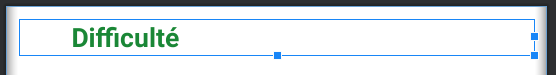
\includegraphics[width=0.7\linewidth]{androidGroupLayout.png}
    \caption{Une simple TextView pour \textit{list\_group.xml}}
\end{figure}

\noindent\underline{\textit{Inflation du layout principal pour accueillir de nouvelles catégories :}}
\begin{minted}[frame=lines,framesep=10pt]{java}
public View getGroupView(int groupPosition, boolean isExpanded, View convertView, 
    ViewGroup parent) {
// On gonfle le layout si nécessaire
if(convertView == null){
    LayoutInflater layoutInflater = (LayoutInflater) 
        context.getSystemService(Context.LAYOUT_INFLATER_SERVICE);
    convertView = layoutInflater.inflate(R.layout.list_group, null);
}
...
\end{minted}
De même, pour afficher les cellules il faut aussi y préciser quel layout utiliser :

\begin{figure}[H]
    \centering
    
\includegraphics[width=0.7\linewidth]{androidCellLayout.png}
    \caption{Quelques TextView pour \textit{cell\_layout.xml}}
\end{figure}

\noindent\underline{\textit{Inflation du layout principal pour accueillir de nouvelles cellules :}}
\begin{minted}[frame=lines,framesep=10pt]{java}
public View getChildView(int groupPosition, int childPosition, boolean isLastChild, 
    View convertView, ViewGroup parent) {
// On gonfle le layout si nécessaire
if(convertView == null){
    LayoutInflater layoutInflater = (LayoutInflater) 
        context.getSystemService(Context.LAYOUT_INFLATER_SERVICE);
    convertView = layoutInflater.inflate(R.layout.cell_layout, null);
}
...
\end{minted}

\subsection{Persistance des données}
Pour que l'utilisateur puisse comparer ses performances actuelles avec ses précédentes tentatives, l'application doit rendre l' historique des statistiques persistante. Comme nos données sont représentées dans un format textuel simple (\hyperref[section:dataformat]{\textcolor{blue}{\underline{voir 4.3.1  Représentation des données}}}), on a choisi de stocker les données dans un fichier text.

\subsubsection{Sauvegarde des données}
A la fermeture de l'activité Main, les données de la liste sont stockées ligne par ligne dans un fichier \textit{stats.txt} à la racine du dossier \textit{Data} attribué par défaut par l' OS Android pour chaque application.\\

\noindent\underline{\textit{Sauvegarde lors de la destruction de l'application :}}
\begin{minted} [frame=lines,framesep=10pt]{java}
protected void onDestroy() {
    // On sauvegarde l'historique des parties quand l'application se ferme
    try {sauvegarderDonnees();} catch (IOException e) {e.printStackTrace();}
    super.onDestroy();
}
...
// Sauvegarde l'historique des parties dans le stockage réservé à l'application
public void sauvegarderDonnees() throws IOException {
    File file = new File(getFilesDir(), "stats.txt");
    // Si le fichier exste on le supprime
    if(file.exists()) file.delete();
    FileOutputStream stream = new FileOutputStream(file);
    try {
        // les stats sont stockés ligne par ligne
        int length = stats.size();
        for(int i=0; i < length-1; i++){
            stream.write((stats.get(i)+"\n").getBytes());
        }
        // Pas de retour à la ligne pour la dernière stat
        stream.write((stats.get(length-1)).getBytes());
    } catch (IOException e) {e.printStackTrace();} finally {
        stream.close();
    }
}
\end{minted}


\subsubsection{Restoration des données}
Au lancement de l'application, si le fichier texte \textit{stats.txt} existe alors on lit le fichier dans son intégralité, comme les données sont stockées ligne par ligne, il suffit de découper la chaîne de caractère lu sur le caractère de retour à la ligne "$\backslash$n". Si le fichier est introuvable, on ne charge rien.\\

\noindent\underline{\textit{Chargement lors du lancement de l'application :}}
\begin{minted} [frame=lines,framesep=10pt]{java}
protected void onCreate(Bundle savedInstanceState) {
...
// On charge l'historique des parties en mémoire
try {chargerDonnees();} catch (IOException e) {e.printStackTrace();}
}

// Charge l'historique des parties dans le stockage réservé à l'application
public void chargerDonnees() throws IOException {
    File file = new File(getFilesDir(), "stats.txt");
    // Si il n'y a pas de sauvegarde on ne charge rien
    if(!file.exists()) return;
    // Lectures du flux de byte
    int length = (int) file.length();
    byte[] bytes = new byte[length];
    FileInputStream in = new FileInputStream(file);
    try {in.read(bytes);} catch (IOException e) {e.printStackTrace();} 
        finally {in.close();}
    // Conversion des bytes en un seul string
    String contents = new String(bytes);
    // Les stats sont stockées ligne par ligne, on découpe et on ajoute en mémoire
    String[] data = contents.split("\n");
    for (int i=0; i < data.length; i++){stats.add(data[i]);}
}
\end{minted}

\section{Conclusion}

Super démineur est un jeu de démineur adapté pour appareils mobiles sur iOs et Android via leurs API standards. Le projet propose 3 niveaux de difficulté, ainsi qu'un historique des parties persistant pour que l'utilisateur compare ses performances actuelles avec ses sessions précédentes.\\

Ce projet a été très enrichissant, dans la mesure où il aura permit de : 
\begin{itemize}
    \item découvrir les spécificités du langage Swift: les optionnelles, la syntaxe objet, etc..
    \item renforcer les connaissances sous Xcode notamment le placement des widget en \% dans le storyboard
    \item gérer un système de contrôle de source : GitHub 
    \item renforcer les connaissances sous Android studio, notamment la description des vues en XML
    \item communiquer entre membres pour imposer des limites réalistes et garder une interface graphique homogène entre iOs et Android
    \item découvrir les mécaniques qui régissent le jeu du démineur 
    \item produire un rapport structuré en \LaTeX \\
\end{itemize}

A l'avenir Super Démineur pourrait intégrer un système de classement en ligne, un niveau de difficulté supplémentaire ou encore des bonus (comme par exemple, révéler la nature d'une case) ainsi que la possibilité de sauvegarder une partie en cours pour la continuer plus-tard.


\newpage

%Bibliographic references
\begin{thebibliography}{9}
\bibitem{androidProf} 
Étienne Payet.
\textit{Programmation Android L3 informatique}. 
Département de mathématiques et d’informatique, Université de La Réunion, 2021.

\bibitem{iosProf} 
Étienne Payet.
\textit{Programmation iOS L3 informatique}. 
Département de mathématiques et d’informatique, Université de La Réunion, 2021.

\bibitem{segmented}
Delacrix Morgan.
\textit{iOS Segmented Control Buttons with RadioGroup in Android}.\\
\url{https://medium.com/bugless/ios-segmented-control-buttons-with-radiogroup-in-android-8968629c200}, consulté le 29 Mai 2021.

\bibitem{listView}
Android Coding.
\textit{How to Create Expandable ListView in Android Studio | ExpandableListView | Android Coding}.\\
\url{https://www.youtube.com/watch?v=E4rrh_WnKMw}, consulté le 28 Mai 2021.

\bibitem{devLibreSegue}
Développeur libre.
\textit{Segue : Passer des Données à travers un View Controller - Xcode 9 et Swift 4}.\\
\url{https://www.youtube.com/watch?v=jYl_MA1TbDg}, consulté le 23 Mai 2021. 

\end{thebibliography}




\end{document}
